\begin{Ponto}{T}
		\label{primeira_tabela_pT}
		\begin{PontoTabela}
			\fileName{CMS024.CMG}
			\fileInit{10/10/0016 13:40:19}
			\fileFim{10/10/0016 13:43:19}
			\fileInfo{59.69}{57.6}{69.6}{0.0}{0.0}
		\end{PontoTabela}
\end{Ponto}
Na \textbf{Figura \ref{primeiro_grafico_pT}} é apresentado o histórico no tempo do nível sonoro do \textbf{Ponto \ponto{T}}, não houve necessidade de tratamento estatístico porque o ruído representado durante a amostragem foi somente do ambiente. \\*
			\begin{figure}[H]
				\centering
				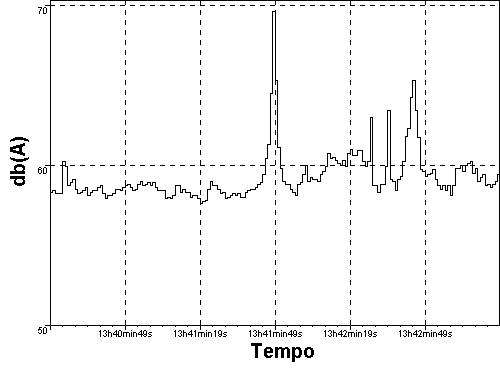
\includegraphics[width=8cm]{pontos/CMS024.PNG}
				\caption{Gráfico sem tratamento}
				\label{primeiro_grafico_pT}
			\end{figure}

\newpage
\begin{Ponto}{T}
		\begin{PontoTabela}
			\fileName{CMS025.CMG}
			\fileInit{10/10/0016 13:44:32}
			\fileFim{10/10/0016 13:47:32}
			\fileInfo{61.65}{59.3}{64.6}{0.0}{0.0}
		\end{PontoTabela}
\end{Ponto}
Na \textbf{Figura \ref{grafico_ref_17}} é apresentado o histórico no tempo do nível sonoro do \textbf{Ponto \ponto{T}}, não houve necessidade de tratamento estatístico porque o ruído representado durante a amostragem foi somente do ambiente. \\*
			\begin{figure}[H]
				\centering
				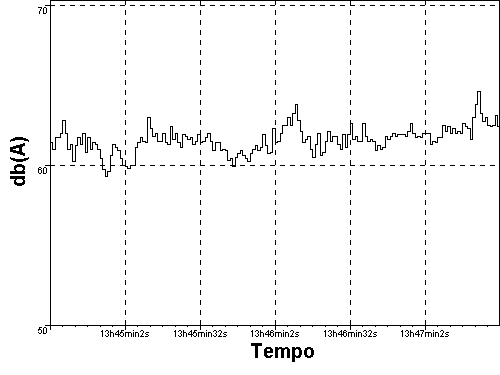
\includegraphics[width=8cm]{pontos/CMS025.PNG}
				\caption{Gráfico sem tratamento}
				\label{grafico_ref_17}
			\end{figure}

\newpage
\begin{Ponto}{T}
		\begin{PontoTabela}
			\fileName{CMS026.CMG}
			\fileInit{10/10/0016 13:48:45}
			\fileFim{10/10/0016 13:51:45}
			\fileInfo{52.65}{50.8}{60.7}{0.0}{0.0}
		\end{PontoTabela}
\end{Ponto}
Na \textbf{Figura \ref{grafico_ref_18}} é apresentado o histórico no tempo do nível sonoro do \textbf{Ponto \ponto{T}}, não houve necessidade de tratamento estatístico porque o ruído representado durante a amostragem foi somente do ambiente. \\*
			\begin{figure}[H]
				\centering
				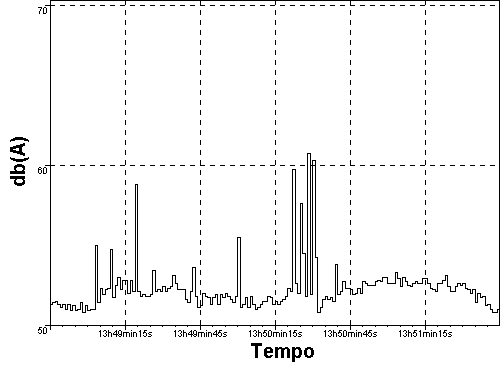
\includegraphics[width=8cm]{pontos/CMS026.PNG}
				\caption{Gráfico sem tratamento}
				\label{grafico_ref_18}
			\end{figure}

\newpage
\begin{Ponto}{T}
		\begin{PontoTabela}
			\fileName{CMS027.CMG}
			\fileInit{10/10/0016 13:52:52}
			\fileFim{10/10/0016 13:55:52}
			\fileInfo{43.29}{41.0}{52.6}{0.0}{0.0}
		\end{PontoTabela}
\end{Ponto}
Na \textbf{Figura \ref{grafico_ref_19}} é apresentado o histórico no tempo do nível sonoro do \textbf{Ponto \ponto{T}}, não houve necessidade de tratamento estatístico porque o ruído representado durante a amostragem foi somente do ambiente. \\*
			\begin{figure}[H]
				\centering
				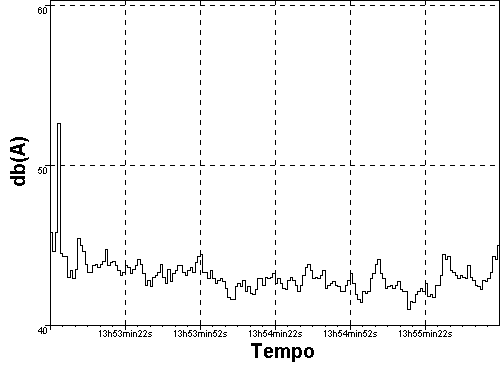
\includegraphics[width=8cm]{pontos/CMS027.PNG}
				\caption{Gráfico sem tratamento}
				\label{grafico_ref_19}
			\end{figure}

\newpage
\begin{Ponto}{T}
		\label{ultima_tabela_pT}
		\begin{PontoTabela}
			\fileName{CMS028.CMG}
			\fileInit{10/10/0016 13:58:20}
			\fileFim{10/10/0016 14:01:20}
			\fileInfo{57.7}{53.8}{62.7}{0.0}{0.0}
		\end{PontoTabela}
\end{Ponto}
Na \textbf{Figura \ref{ultimo_grafico_pT}} é apresentado o histórico no tempo do nível sonoro do \textbf{Ponto \ponto{T}}, não houve necessidade de tratamento estatístico porque o ruído representado durante a amostragem foi somente do ambiente. \\*
			\begin{figure}[H]
				\centering
				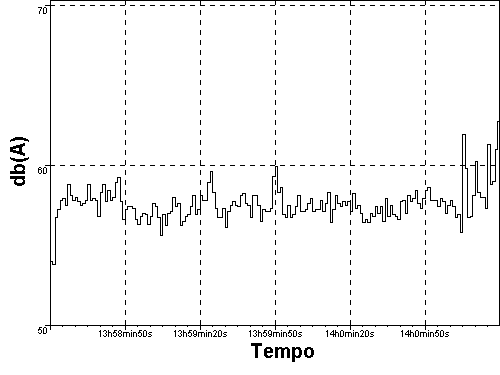
\includegraphics[width=8cm]{pontos/CMS028.PNG}
				\caption{Gráfico sem tratamento}
				\label{ultimo_grafico_pT}
			\end{figure}

\newpage
